\chapter{トポロジー導関数の定義}

\section{トポロジー導関数の定義}
\begin{figure}[ht]
	\begin{center}
		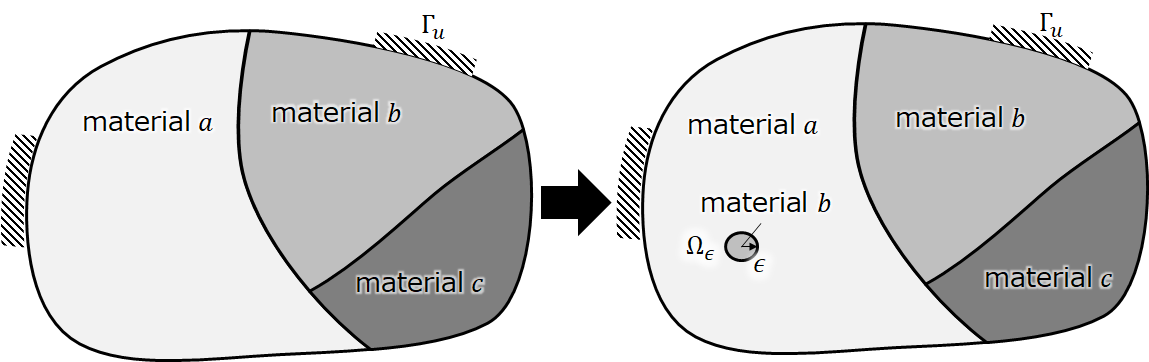
\includegraphics[width=13cm]{./figures/GeneHole.png}
		\caption{Definition of topological derivative}
		\label{fig:GeneHole}
	\end{center}
\end{figure}

トポロジー導関数は設計領域中で定義される関数で,各点$\bm{x}$を中心とする微小な円領域が,別の材料に置き換わった時の目的関数の感度を表す.
図\ref{fig:GeneHole}のように,材料$a$の占める領域中の位置$\bm{x}=\bm{z}$を中心とする微小な円領域に,材料$b$が生じた際のトポロジー導関数$D_{T}F^{a\rightarrow b}(\bm{z})$は以下のように定義される.
\begin{align}
D_{T}F^{a\rightarrow b}(\bm{z})=\lim_{\epsilon\rightarrow 0}\frac{\delta F^{a\rightarrow b}(\bm{z})}{g(\epsilon)}
\end{align}
ここで,$\delta F^{a\rightarrow b}$は目的関数の変化,$g(\epsilon)$は極限値が存在するように定義される$\epsilon$の関数である.
一般的に次式のように$\Omega_{\epsilon}$の測度で定義される.
\begin{align}
g(\epsilon)=&\pi\epsilon^2 \hspace{1cm}\text{(for 2D)} \\
=&\frac{3}{4}\pi\epsilon^3 \hspace{0.8cm}\text{(for 3D)}
\end{align}

\section{Topological-Shape Sensitivity Method}

\begin{figure}[ht]
	\begin{center}
		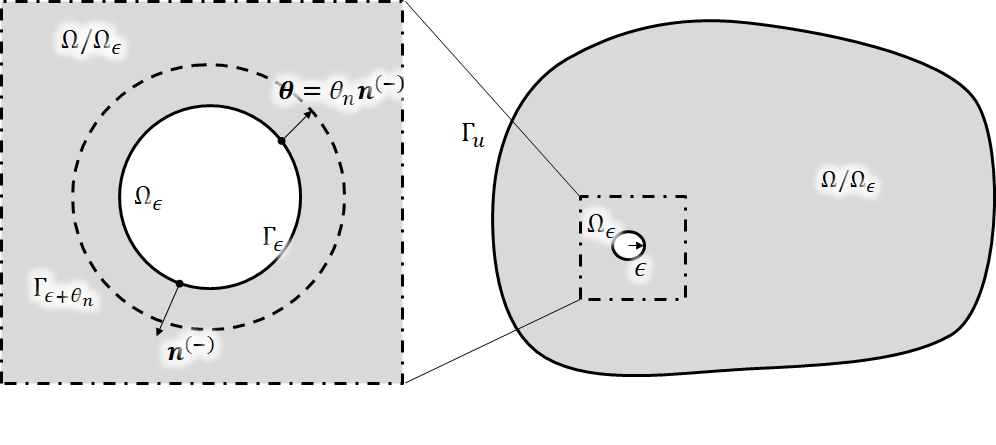
\includegraphics[width=13cm]{./figures/TSSM.png}
		\caption{Concept of Topological-Shape Sensitivity Method}
		\label{fig:TSSM}
	\end{center}
\end{figure}

Novotny et al.は形状微分の極限をとることでトポロジー導関数を導出する方法を提案した.
形状微分とは構造の境界が微小量移動した時の目的関数の感度である.

$\bm{\theta}(\bm{x})$方向に形状が微小変動するとき,領域写像$\psi_{s}(\bm{x})$は次式のように表される.
\begin{align}
\psi_{s}(\bm{x})=\bm{x}+s\bm{\theta}(\bm{x})
\end{align}
この時,形状微分$DF(\Omega)\cdot\bm{\theta}$は以下のように定義される.
\begin{align}
DF(\Omega)\cdot\bm{\theta}=\frac{d}{ds}F(\psi_{s}(\Omega))
\end{align}
図\ref{fig:TSSM}のように半径$\epsilon$の空洞$\Omega_{\epsilon}$が物体領域$\Omega/\Omega_{\epsilon}$内向き法線$\bm{n}^{(-)}$方向に膨張する時,つまり
\begin{align}
\bm{\theta}=&\theta_{n}\bm{n}^{(-)}	\hspace{1cm}\text{on}\hspace{0.3cm}\Gamma_{\epsilon}\\
\bm{\theta}=&\bm{0}					\hspace{1.8cm}\text{on}\hspace{0.3cm}\Gamma/\Gamma_{\epsilon}
\end{align}
となる時の形状微分を考える.$\theta_{n}$は正の値をとる定数である.
トポロジー導関数は以下のように$\epsilon\rightarrow0$の極限をとることで得られる.
\begin{align}
D_{T}F=\lim_{\epsilon\rightarrow 0}\frac{1}{g'(\epsilon)|\theta_{n}|}\Bigl(DF\cdot \bm{\theta}\Bigr)(\epsilon)
\label{eq:TSSen}
\end{align}
ただし,$g'(\epsilon)$は$g(\epsilon)$の$\epsilon$に関する微分を表す.
このような,形状微分に基づくトポロジー導関数の導出方法をTopological-Shape Sensitivity Methodと呼び,
以下のプロセスで導出する.
まず,形状微分$DF\cdot \bm{\theta}$を求める.
次に,$\epsilon\rightarrow0$とした時の状態場や随伴場の漸近的な振る舞いを調べる.
その結果を式\eqref{eq:TSSen}に代入することでトポロジー導関数を導出する.
